\IEEEPARstart{A}{ccording} 
to the World Health Organization, ``285 million people are estimated
to be visually impaired worldwide.''~\cite{WHOvisuallyimpaired}
Several technologies such as automatic text readers, Braille note
makers, and navigation assist canes have been developed to assist the
visually impaired. Concurrent advances in computer vision and hardware
technologies provides opportunities for a visual-assist system that
can be used in multiple contexts.

As part of the Visual Cortex on Silicon program, we have been
developing algorithms, hardware platforms and interfaces to assist the
visually impaired with a focus on grocery shopping. Grocery shopping
is an essential activity in our daily lives that involves various
interconnected activities. These include checking the pantry for
current inventory, making a shopping list based on planned meals,
getting to the store, and making opportunistic and impulsive purchases
in response to signage at the store. Each one of these activities
poses a significant challenge without visual cues.  Consequently, our
Third-Eye prototype enables a combination of hardware software
mechanisms to interpret these visual cues and communicate them to a
visually impaired user as verbal or vibrational feedback.

A potpourri of different vision algorithms spanning brain-inspired
algorithms, structured feature extraction techniques and deep learning
approaches is used to support the automation of the different visual
tasks. While both the origins and implementations of these algorithms
are diverse, many share a common feature in that they work to reduce
the potentially vast search spaces that vision problems can
involve. Brain-inspired solutions, such as saliency algorithms, help
to focus attention onto only specific parts of a complex image,
thereby significantly reducing the computational effort to process the
input and can act as a filter for subsequent steps.  Other
brain-inspired solutions such as GIST provide a contextual reference
to the image and prime the decision making with that information,
thereby filtering the model space of likely objects to be found.

In composition, these algorithms can be very powerful. Consider
searching for an object in an aisle. First, steps such as saliency can
help you reduce the effort spent examining the floor, empty shelves
and other parts of an image that don't strongly register as potential
grocery objects. Then, by understanding the context of specific
grocery aisles instead of the entire store, complexity can be further
pruned.  For example, if milk is in your shopping list, the system can
be primed to only search for milk when you arrive at the dairy aisle
and to furthermore limit the number of distinct types of possible
objects considered during classification to those likely to be in a
dairy aisle. Such optimizations considerably reduce the computational
load on the assistive vision system. In conjunction with these
algorithmic advances, we have developed customized hardware solutions
to make these operations more power-efficient as well as provide
real-time feedback to the user.

\begin{figure}[!htb]
\centering
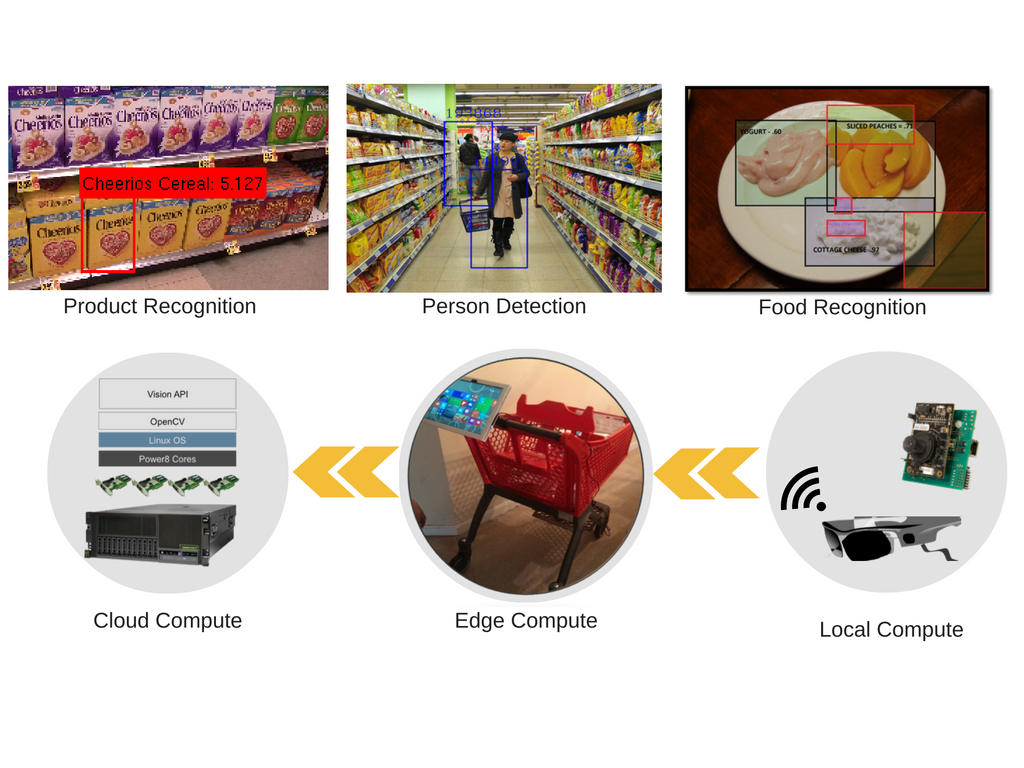
\includegraphics[width=0.9\linewidth,trim={0 80 0 0},clip]{introduction.png}
\caption{Applications and underlying technologies}
\label{fig:introduction}
\end{figure} 
%  Consequently, this serves as a good region of interest extractor
%  for subsequent steps.

The rest of this article describes the following set of visual
assistive functions: (1) Identifying objects in a pantry including
misplaced items; (2) Identifying other shoppers when navigating in the
store or when navigating to the stores; (3) Locating packaged objects
from the grocery shelf and picking them; (4) Assisting in identifying
items from prepared food sections. 

%For each of these tasks we consider not only the computer vision
%aspects of the problem, but also the practical embodiment of a
%complex system spanning wearables, edge, and cloud computing
%platforms that must solve the last mile issues of a real, usable
%consumer device.
